% !TEX root = ../main.tex
\section{Nuclei-proton Interactions}

Nucleon-nucleon and nucleus-nucleus reactions are governed by the strong force, a short-range interaction. Unlike leptons and photons, nucleons and nuclei are extended objects with radii approximately $R_N \sim 1.2 A^{1/3}$~fm. This results in interaction cross-sections of the order of the geometrical cross-section $\sigma_{\rm geom} \simeq \pi R_N^2 \simeq 45 A^{2/3}$~mb\footnote{As reference value $1~\text{mb} = 10^{-27}~\text{cm}^2 \sim \frac{\sigma_{\rm T}}{500}$.}, which is a valid rule of thumb~\cite{Letaw1983apjs}.

Therefore, in regions with increased target density, such as the inner regions of starburst galaxies or galactic molecular clouds, one can estimate the timescale of high-energy nuclei interacting with gas targets as
%
\[
\tau \simeq \frac{1}{n_{\rm t} \sigma_{\rm geo} c} \simeq 25 \, A^{-2/3} \left( \frac{n_{\rm H}}{\text{cm}^{-3}} \right)^{-1}~\text{Myr}
\]
%
This timescale proves competitive when compared to other processes, such as particle escape or other forms of energy loss.

A significant portion of astrophysical gamma rays and neutrinos originate from the decay of pions, which are generated in interstellar collisions where protons serve as both targets and projectiles.

High-energy proton interactions primarily result in the following final states:
%
\[
p + p \rightarrow 
\begin{cases}
p + p + \pi^0 \\
p + n + \pi^+ \\
p + p + \pi^+ + \pi^- 
\end{cases}
\]

The production of neutral pions $\pi^0$ leads to gamma-ray radiation through the decay 
%
\[ 
\pi^0 \rightarrow {\color{red}\gamma} + {\color{red}\gamma} 
\]

The decay of charged pions, followed by the secondary muon decay, generates a total of 3 neutrinos in the final state as 
%
\begin{eqnarray*}
\pi^+ & \rightarrow & {\color{red}\nu_\mu} + \mu^+ \\
& & \hphantom{\nu_\mu + l} \drsh \, e^+ + {\color{red}\bar \nu_\mu} + {\color{red}\nu_e} \\
\pi^- & \rightarrow & {\color{red}\bar \nu_\mu} + \mu^- \\
& &  \hphantom{\bar \nu_\mu + l} \drsh \, e^- + {\color{red}\nu_\mu} + {\color{red}\bar \nu_e} 
\end{eqnarray*}

In this scenario, the same mechanism that generates high-energy photons also produces neutrinos. Consequently, the presence of neutrinos serves as a definitive indicator of hadronic processes, distinguishing them from processes primarily involving leptons, which do not produce neutrinos.

The energy threshold for $\pi^0$-production in the proton-proton collision is determined by
%
\[
2 m_p^2 + 2 E^{\rm th}_p m_p = \left(2 m_p + m_{\pi^0} \right)^2
\]
%
where $E^{\rm th}_p$ is the proton energy threshold in the LAB frame.

Using $m_p = 0.938$~GeV, and $m_{\pi^0} = 0.135$~GeV, one obtains
%
\begin{equation}
E_p^{\rm th} = m_p + 2 m_\pi + \frac{m_\pi^2}{2 m_p} \simeq 1.22~\text{GeV}
\end{equation}
%
or, in terms of kinetic energy,
%
\begin{equation}
T_p^{\rm th} = E_p^{\rm th} - m_p \simeq 280~\text{MeV}
\end{equation}

The inelastic cross-section for proton-proton collisions, denoted as \(\sigma_{\rm pp}\), has been accurately measured in terrestrial accelerators, with a clear dependence on the proton energy in the laboratory frame. This cross-section rapidly increases from the particle production threshold, reaching several tens of mb's at proton energies of a few GeV, and thereafter exhibits a more gradual increase with energy.

A convenient parametrization for the total inelastic cross-section can be found in~\cite{Kelner2006prd}
%
\[
\sigma_{\rm inel} = (34.3 + 1.88~L + 0.25~L^2) \left[ 1 - \left( \frac{E^{\rm th}_p	}{E_p} \right)^4 \right]^2 \, \text{mb}
\]
%
where $L \equiv \ln (E_p / \text{TeV} )$.

\begin{figure}[t]
\centering
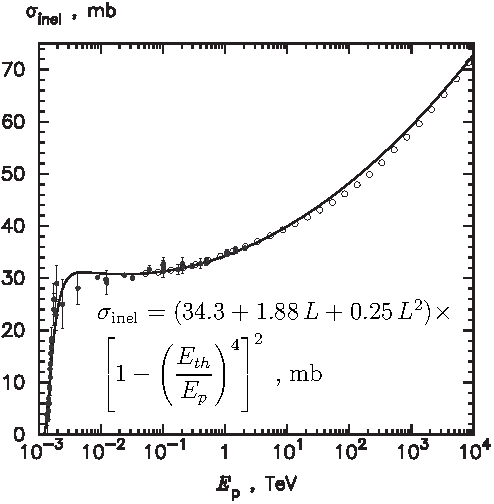
\includegraphics[width=0.5\textwidth]{figures/KelnerAharonian11.pdf}
\caption{Kelner Aharonian~\cite{Kelner2006prd}}
\end{figure}

The parametrization of experimental data for pion production in proton-proton collisions is detailed in~\cite{Norbury2009nimpb}:
%
\begin{eqnarray*}
\sigma_{pp\rightarrow \pi^+ X} & = & \left( 0.00717 + 0.0652 \frac{\log T_p}{T_p} + \frac{0.162}{T_p^2} \right)^{-1}~\text{mb} \\
\sigma_{pp\rightarrow \pi^- X} & = & \left( 0.00456 + \frac{0.0846}{T_p^{0.5}} + \frac{0.577}{T_p^{1.5}} \right)^{-1}~\text{mb} \\
\sigma_{pp\rightarrow \pi^0 X} & = & \left( 0.007 + 0.1 \frac{\log T_p}{T_p} + \frac{0.3}{T^2} \right)^{-1}~\text{mb} 
\end{eqnarray*}
%
where $T_p$ is the kinetic energy of the proton in the LAB frame in units of GeV.

An interesting characteristic of pion production is that the channels appear to follow the relation:
%
\[ 
\sigma_{pp\rightarrow \pi^0 X}  \simeq \frac{1}{2} (\sigma_{pp\rightarrow \pi^+ X}  + \sigma_{pp\rightarrow \pi^- X}) 
\]

\begin{figure}[t]
\centering
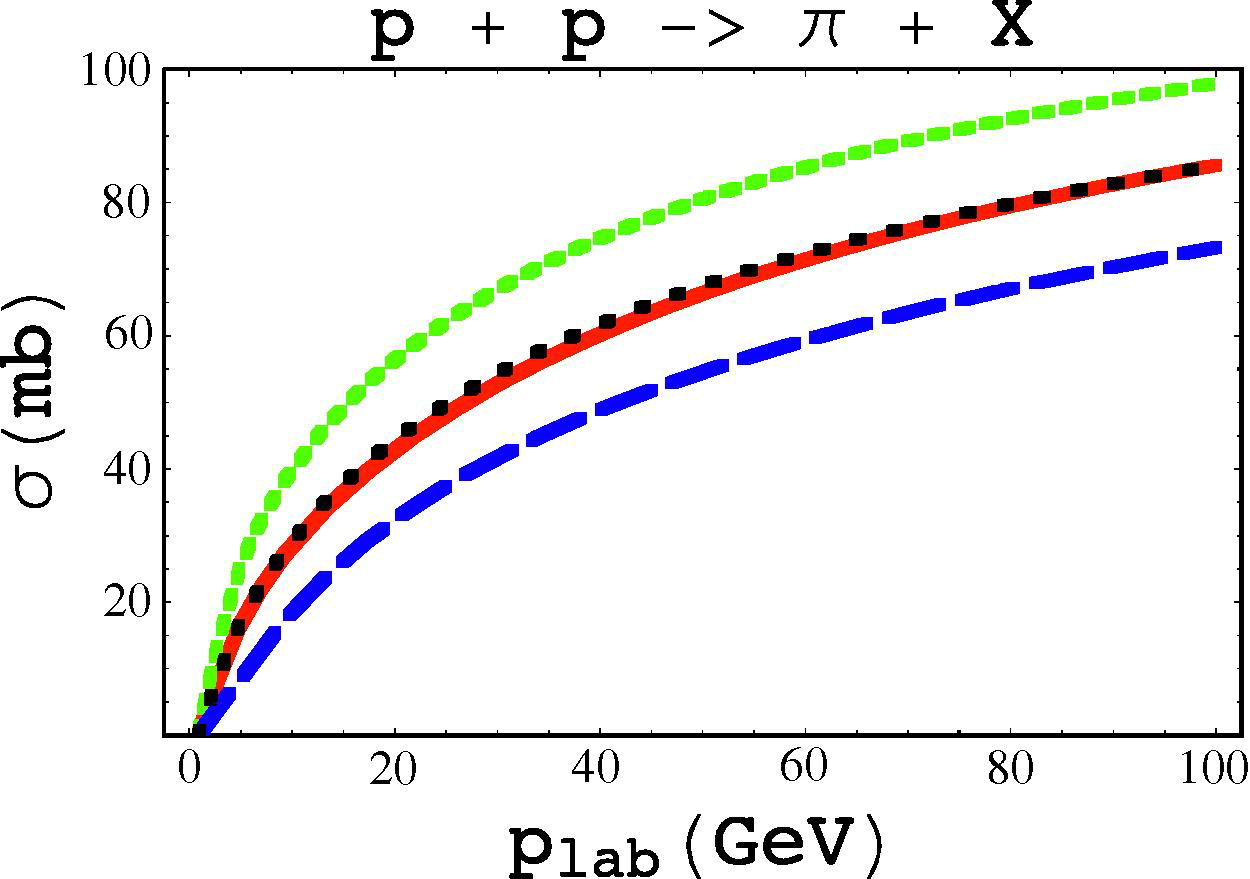
\includegraphics[width=0.5\textwidth]{figures/Norbury2009.jpg}
\caption{Parameterized inclusive cross sections for pion production in proton-proton collisions. The green dotted line is X. The red solid line is X. The blue long dashed line is X. The black dotted curve is calculated from X. ~\cite{Norbury2009nimpb}}
\end{figure}

It's noteworthy that the threshold for the \( p+p \rightarrow \pi^- + X \) reaction occurs at \( T_p \simeq 600 \) MeV, attributed to the presence of two new particles in the final state. This threshold is higher compared to the \( \pi^+ \) production, which has a threshold of \( T_b \simeq 289 \) MeV. This difference accounts for the consistently larger cross-section of \( \pi^+ \) compared to \( \pi^- \).

Consequently, this asymmetry in pion production leads to a greater secondary production of positrons than electrons in cosmic rays~\cite{Moskalenko1998apj}.

The inelasticity\footnote{The inelasticity is the fraction energy loss of the initial proton.} factor for this process, involving proton energies in the GeV-TeV range, is approximately \( K_{\pi^0} \simeq 0.17 \). Utilizing this value, we can derive the resulting spectrum from proton-proton (pp) interactions. For this purpose, we employ the delta-function approximation, expressed as \( T_\pi \simeq K_\pi T_p \).

We begin by introducing the pion emissivity as the number of pions produced per unit time, volume, and energy, denoted as \( q_\pi = \frac{dN_\pi}{dt dV dE} \). Consequently,
%
\[
q_\pi (E_\pi) = c n_{\rm H} \int \delta(T_\pi - K_\pi T_p) \sigma_{pp} (E_p) {N_p(E_p)} dE_p
\]
%
where...

Follows,
\[
q_\pi (E_\pi) \simeq c n_{\rm H} \int \delta(T_\pi - K_\pi E_p + K_\pi m_p) \sigma_{pp}(E_p) {N_p(E_p)} dE_p
\]
%
integrating over the $\delta$-function we arrive to
%
\[
q_\pi (E_\pi) \simeq \frac{c n_{\rm H}}{K_\pi} \sigma_{pp} \left(\frac{T_\pi}{K_\pi} + m_p \right) N_p \! \left(\frac{T_\pi}{K_\pi} + m_p \right)
\]

In the high-energy limit, where the mass of the pion can be disregarded,
%
\[
q_\pi (E_\pi) \underset{E_\pi \gg m_\pi}{\simeq} \frac{c n_{\rm H}}{K_\pi} \sigma_{pp}\left(\frac{E_\pi}{K_\pi}\right) N_p \! \left(\frac{E_\pi}{K_\pi} \right)
\]

As a result, the pion spectrum closely mirrors the shape of the parent proton spectrum, albeit shifted to a lower energy by a factor of \( K_\pi \).

\subsection{The $\pi^0$ gamma-ray spectrum}

The decay of \(\pi^0\) into two gamma photons occurs almost instantaneously. Due to momentum conservation, these photons are emitted in opposite directions (back-to-back) in the frame where the \(\pi^0\) is at rest (CoM). 
%
Energy conservation dictates that in this same frame, each photon carries an energy of \(E^\prime_\gamma = \frac{m_\pi}{2}\).

In the LAB frame, where the pion moves with velocity $\beta_\pi$,
%
\begin{equation}\label{eq:egamma}
E_\gamma = \frac{m_\pi}{2} \gamma_\pi (1+\beta_\pi \cos \theta^\prime)
\end{equation}
%
where $\theta^\prime$ is the angle between photons and the direction of the pion.

The minimum and maximum photon energies are determined by varying the angle \(\theta\) within its permissible range from -1 to 1:
%
\[
E_{\gamma}^{\rm min(max)} = \frac{m_\pi}{2} \gamma_\pi (1 \mp \beta_\pi)
\]

In the non-relativistic limit, where \(\beta \simeq 0\) and correspondingly \(\gamma \simeq 1\), both the minimum and maximum photon energies converge to \( E_{\gamma}^{\rm min} \simeq E_{\gamma}^{\rm max} \simeq \frac{m_\pi}{2} \).

Conversely, in the ultra-relativistic limit where \(\beta \simeq 1\) and \(\gamma \rightarrow \infty\), the minimum photon energy approaches \( E_\gamma^{\rm min} \simeq 0 \), while the maximum energy escalates to \( E_\gamma^{\rm max} \simeq E_\pi \rightarrow \infty \).

From Eq.~\ref{eq:egamma}, we deduce a relationship between the photon energy and the emission angle, leading to
%
\[
dE_\gamma = \frac{m_\pi}{2} \gamma_\pi \beta_\pi \, d\!\cos\theta^\prime
\]

Given that the pion is a scalar particle, its decay products are emitted isotropically. This is expressed as:
%
\[
\int d\Omega \frac{dN}{d\Omega} = 1 
\]
%
from this, we obtain~\footnote{Remind: $d\Omega = \sin \theta d\theta d\phi \rightarrow \langle d\Omega \rangle_\phi = 2 \pi d\cos\theta$}:
%
\[
\frac{dN}{d\Omega} = \frac{1}{4\pi} \rightarrow dN = \frac{1}{2} \, d\!\cos\theta^\prime
\]

Combined together, we conclude
%
\begin{remark}
\[
\frac{dN}{dE_\gamma} = \frac{1}{m_\pi \gamma \beta} = \frac{1}{(E^2_\pi - m_\pi^2)^{1/2}}
\]
\end{remark}

Therefore, after boosted for the energy of the emitting $\pi^0$, the probability to emit a photon of energy $E_\gamma$  is uniformly distributed in energy space between, in the relativistic limit, \(E_{\rm min} \simeq 0\) and \(E_{\rm max} \simeq E_\pi\). Essentially, one can expect a \emph{box-like} spectrum within this range.

We now move to calculate the mean energy using a logarithmic representation, that is:
%
\[
\langle \log E \rangle 
= \frac{1}{2} \left[ \log E_{\rm \gamma, min} + \log E_{\rm \gamma, max} \right] 
= \log \left[ \frac{E_\pi^2}{4} (1-\beta_\pi^2) \right]^{1/2} = \log \left(\frac{m_\pi}{2}\right)
\]

This implies that in a \emph{logarithmic scale}, the central point of the interval is equivalent to half the pion's rest mass, independent of \(E_\pi\).

The resulting spectrum is composed of a weighted sum of such \emph{box-like} distributions. Since each component of this distribution is symmetrically centered around \( m_\pi / 2 \), the photon distribution will peak at \( \log(m_\pi / 2) \).

Consequently, the gamma-ray spectrum consistently exhibits a prominent feature at approximately \( 67.5 \) MeV, regardless of the pion spectrum and, by extension, the spectrum of the parent protons.
%
A characteristic \emph{bump} in the energy spectrum, peaking at around $\sim$70 MeV, followed by a decline, might serve as a clear identifier of $\gamma$-rays originating from hadronic processes.

\begin{figure}[!t]
\centering
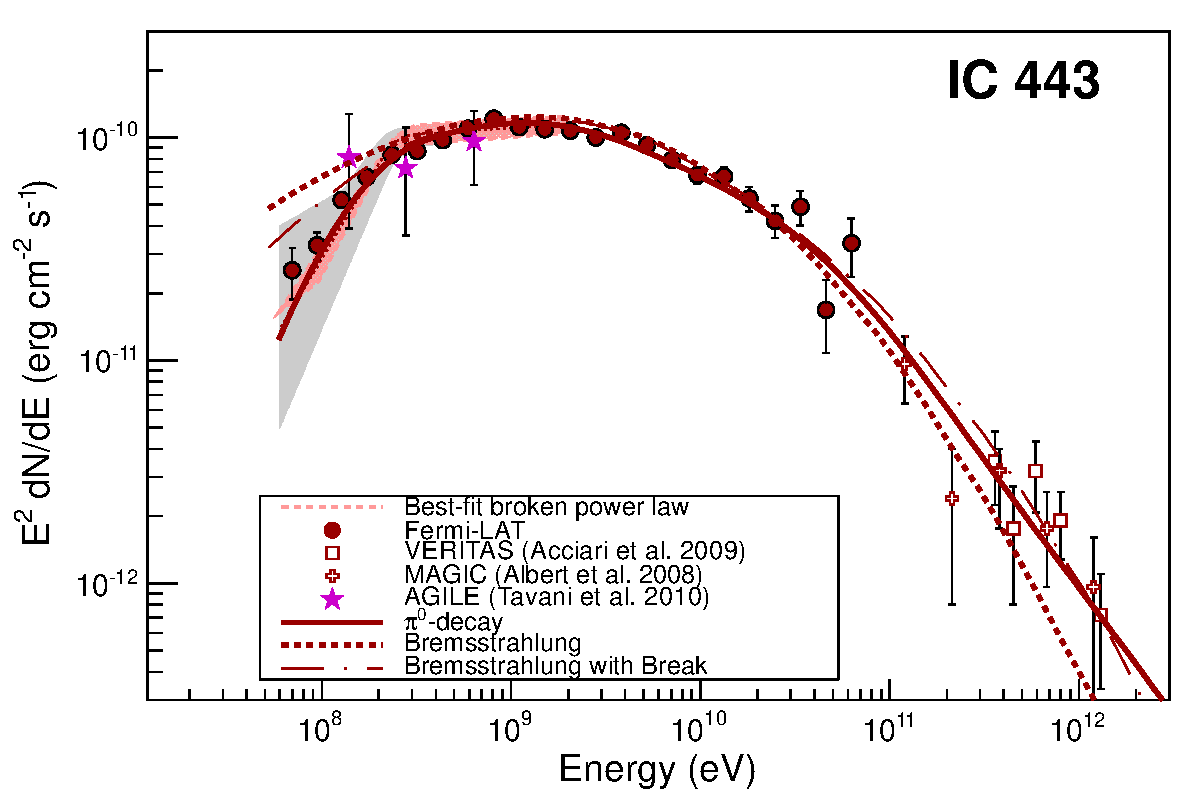
\includegraphics[width=0.45\textwidth]{figures/1231160fig2a.pdf}
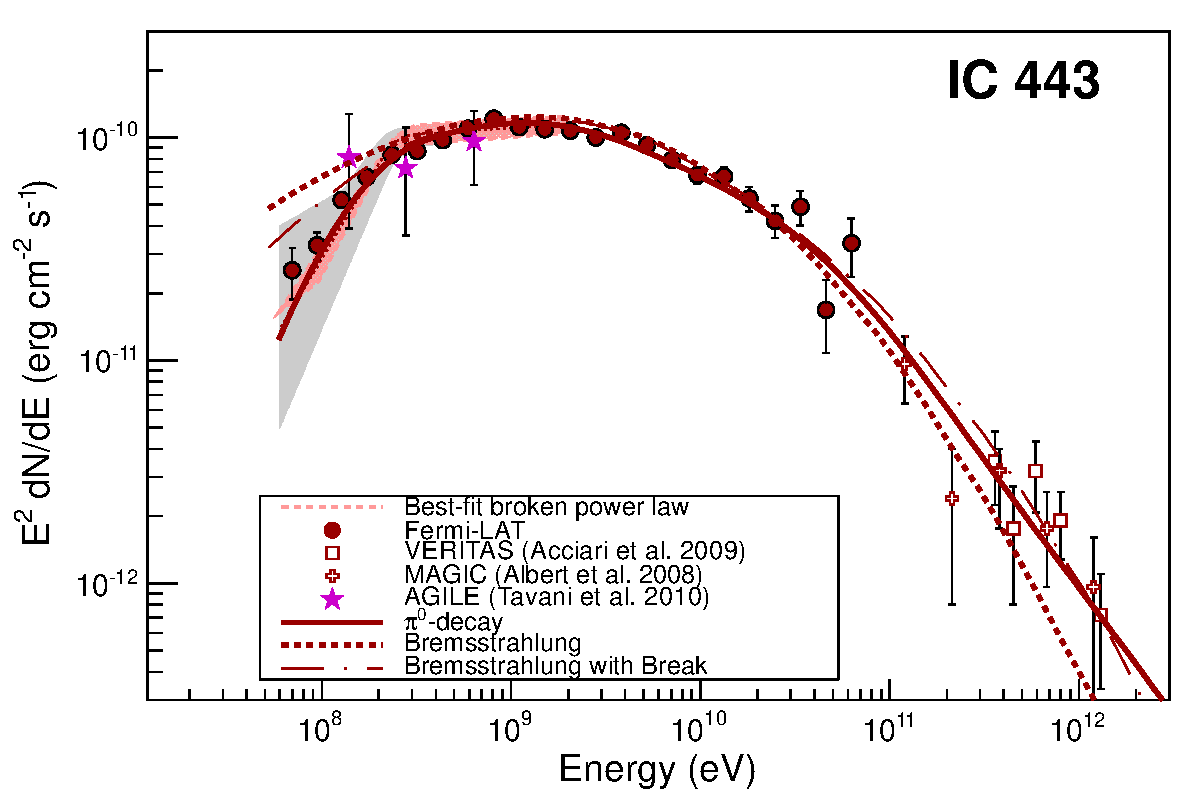
\includegraphics[width=0.45\textwidth]{figures/1231160fig2a.pdf}
\caption{In 2013 FERMI detected a feature compatible with the pion-bump in two old SNRs in interaction with Molecular Cloud~\cite{Ackermann2013sci}}
\end{figure}

Observe that \( E_{\rm \gamma, min} + E_{\rm \gamma, max} = E_\pi \) and \( E_{\rm \gamma, min} E_{\rm \gamma, max} = \frac{m_\pi^2}{4} \). Hence, we can express this as:
%
\[
E_\pi = E_{\rm \gamma, min} + E_{\rm \gamma, max} = E_{\rm \gamma, max} + \frac{m_\pi^2}{4E_{\rm \gamma, min}}
\]

As a result, for a given photon energy \( E_\gamma \), the minimum pion energy required to produce a photon of energy \( E_\gamma \) occurs when \( E_{\rm \gamma,min} = E_{\rm \gamma,max} = E_\gamma \), thereby:
%
\[
E_{\rm \pi, min} = E_\gamma + \frac{m_\pi^2}{4 E_\gamma}
\]

This relationship helps in determining the lower limit of the pion energy necessary for generating a photon of a specified energy \( E_\gamma \). In fact, the $\gamma$-ray emissivity can be written as
%
\[
q_\gamma(E_\gamma) = 2 \int_{E_{\rm \pi, min}}^\infty dE_\pi q(E_\pi) \frac{dN}{dE_\gamma} = 
2 \int_{E_\gamma + \frac{m_\pi^2}{4 E_\gamma}}^\infty dE_\pi \frac{q(E_\pi)}{(E_\pi^2 - m_\pi^2)^{1/2}} \simeq 2 \int_{E_\gamma}^\infty \frac{dE_\pi}{E_\pi} q_\pi(E_\pi)
\]
%
where the final expression holds true at very high energies, a regime in which the pion mass can be considered negligible.

Even at this early stage, we can note that the gamma-ray spectrum maintains the same spectral index as the protons, albeit shifted in energy by a factor of approximately \( K_\pi / 2 \).

To advance, let's calculate the pion emissivity as follows:
%
\[
q(E_\pi) = c n_{\rm H} \int_{E_\pi}^\infty dE_p N_p (E_p) \frac{d\sigma}{dE_\pi}(E_p, E_\pi)
\]
%
where $\frac{d\sigma}{dE_\pi}$ is the differential pion production cross section, $n_{\rm H}$ is the average matter density, \dots

The \emph{differential} cross-section for pion production in proton-proton interactions can be expressed in terms of the total inclusive cross-section as follows:
%
\[
\frac{d\sigma}{dE_\pi}(E_p, E_\pi) = \sigma_{pp}(E_p) \frac{f(E_p, E_\pi)}{E_\pi}
\]

Here, \(f\) is an auxiliary function designed to fit experimental data, fulfilling the condition $\int_{E_{\rm \pi,min}}^{E_{\rm \pi,max}} \frac{dE_\pi}{E_\pi} f(E_p, E_\pi) = 1$. 
%
Moreover, it has been observed that $f$ depends on \(E_p\) and \(E_\pi\) through the combined parameter \(x = E_\pi / E_p\). 

A parametrization of \(f(x)\) is provided in the literature~\cite{Cavasinni2006aph}:
%
\[
f(x) = 0.67 (1-x)^{3.5} + 0.5 \exp(-18 x)
\]

The proton intensity, as observed in cosmic radiation, is assumed to adhere to a power-law dependence on energy
%
\[
I_p(E_p) = I_0 \left(\frac{E_p}{E_0}\right)^{-\alpha}
\]

Upon substitution, the pion emissivity simplifies to
%
 \[
q(E_\pi) \simeq 4 \pi n_{\rm H} I_0 \sigma_0 \int_{E_\pi}^\infty \frac{dE_p}{E_\pi} \left(\frac{E_p}{E_0} \right)^{-\alpha} f(x) = 4 \pi n_{\rm H} I_0 \sigma_0 \left(\frac{E_p}{E_0} \right)^{-\alpha} \underbrace{K_\pi^{-\alpha} \int_0^1 dx x^{\alpha-2} f(x)}_{Y(\alpha)}
\]
%
where $Y(\alpha)$ is the spectrum-weighted yield of pions produced from a power-law proton spectrum of spectral index $\alpha$.

Finally, for a proton population following a power-law distribution, the photon emissivity can be expressed as:
%
\begin{remark}
\[
q(E_\gamma) = 2 \int_{E_\gamma}^\infty \frac{dE_\pi}{E_\pi} q(E_\pi) = 
8 \pi n_{\rm H} I_0 \sigma_0 Y(\alpha) \int_{E_\gamma}^\infty \frac{dE_\pi}{E_\pi}  \left(\frac{E_\pi}{E_0} \right)^{-\alpha}
= \frac{8 \pi}{\alpha} n_{\rm H}  \sigma_0 Y(\alpha) I_p\left(E_\gamma \right)
\]
\end{remark}

The final expression for \( q(E_\gamma) \) highlights the significant correlation between the spectral index of the proton energy spectrum and that of gamma rays, and by extension, with neutrinos:
%
\[
\alpha_p \simeq \alpha_\gamma \simeq \alpha_\nu
\]

In contrast to IC scattering, this relationship aids in differentiating between the two processes. Specifically, the gamma-ray spectrum resulting from hadronic processes more closely mirrors the spectral index of the parent protons, whereas gamma rays produced via IC scattering exhibit a comparatively flatter behavior relative to their parent electrons $E^{\frac{-\alpha-1}{2}}$.

\begin{problem}
Compute the shape of $q_\gamma(E_\gamma)$ using the fitting formula of Eq.~(1) in 1302.3307 and using the $\delta$-function approximation. Plot $q_\gamma(E_\gamma)$ in linear scale and $E_\gamma^2q_\gamma(E_\gamma)$ in log-log one. 
\end{problem}

To demonstrate the utility of these results, we estimate the expected diffuse galactic gamma-ray background, which arises from the scattering of cosmic rays through proton-proton interactions within our Galaxy.

Assuming the local cosmic rays are a fair representation of their overall density in the Galaxy, we can express the gamma-ray intensity as follows:
%
\[
I_\gamma(E_\gamma) = \frac{1}{4\pi} \int_{\rm los} \! ds \, q(E_\gamma) = \frac{2}{\alpha} N_{\rm H} \sigma_0 Y(\alpha) I_p(K_\gamma E_p) 
\]

Here, \( N_{\rm H} = \int_{\rm los} \! ds \, n_{\rm H} \) represents the column density of the gas, and \( K_\gamma = K_\pi / 2 \sim 0.1 \).

Consequently, the energy squared times the gamma-ray intensity is given by:
%
\[
E_\gamma^2 I_\gamma = \frac{2}{\alpha} N_{\rm H} \sigma_0 Y(\alpha) K_\gamma^2 \left[ E_p^2 I_p(E_p) \right]_{E_p = E_\gamma / K_\gamma}
\]

To calculate the gamma-ray intensity at 1 GeV, we utilize a gas column density along the Galactic plane of \( N_{\rm H} \simeq 10^{23} \) cm\(^{-2}\), as inferred from radio observations. The proton intensity, derived from direct measurements, is:
%
\[
\left[ E_p^2 I_p(E_p) \right]_{E_p = 10 \text{ GeV}} \simeq 2 \times 10^3 \text{ GeV m}^{-2} \text{s}^{-1} \text{sr}^{-1}
\]

Employing a cross-section \( \sigma_0 \simeq 30 \) mb, and {\color{red}a value of \( Y(\alpha) \) around 10}\footnote{Recompute...}, we find:
%
\[
E_\gamma^2 I_\gamma \simeq 5 \times 10^{-5} \text{ GeV cm}^{-2} \text{s}^{-1} \text{sr}^{-1}
\]

This estimate closely aligns with the average value of the diffuse emission measured around the Galactic plane (within \( |b| < 5.0 \) degrees) for \( E_\gamma \simeq \) GeV, for instance, by the Fermi-LAT.

This correlation strongly suggests that the diffuse galactic gamma-ray background is likely the result of pp interactions within our Galaxy.

%%% SUBSECTION %%%
\section{Nuclei-$\gamma$ Interactions}

In the vicinity of astrophysical sources, there is often a high density of photons spanning a range of wavelengths, including radio, infrared, visible, and ultraviolet.

While the cross-section for \(\gamma\)-proton interactions is typically two orders of magnitude smaller than that of pp interactions, in certain astrophysical environments, secondary meson production via photoproduction can be substantially higher than that from pp interactions. This increased probability is due to the much greater number density of ambient photons \(n_\gamma\) compared to the number density of matter in the environment.

In the interaction of nuclei with radiation fields, the dominant mechanism is photo-pion production, as exemplified by the following processes:
%
\[
p + \gamma \rightarrow \Delta^+ \rightarrow
\begin{cases} 
p + \pi^0 \\
n + \pi^+
\end{cases}
\]

The subsequent decay of these pions follows the same pattern as previously discussed.

At very high energies, multi-pion production becomes significant, represented by:
%
\[
p + \gamma \rightarrow p + a \pi^0 + b ( \pi^+ + \pi^-)
\]
%
where $a$ and $b$ are multiplicities...

For UHECRs, a competitive process for energy loss is pair production:
%
\[
p + \gamma \rightarrow p + e^+ + e^-
\]

The thresholds for these two processes can be calculated as:
%
\[
E_p^\pi = \frac{m_\pi^2 + 2 m_\pi m_p}{2 \epsilon (1 - \cos \theta)} \simeq 7 \times 10^9 \, \text{eV}
\]
and
\[
E_p^{ee} = \frac{4 m_e^2 + 8 m_e m_p}{2\epsilon (1 - \cos\theta)} \simeq 6 \times 10^{17} \, \text{eV}
\]

Notice that both energy thresholds are inversely proportional to \(\epsilon\). This implies that a lower energy threshold corresponds to interactions with a photon field of higher energy.

For pion production, the typical cross-section as measured in laboratory is:
%
\[
\sigma_{p\gamma} \simeq 
\begin{cases}
340 \, \mu\text{b} & 200 \, \text{MeV} \lesssim E^\prime_\gamma \lesssim 500 \, \text{MeV} \\
120 \, \mu\text{b} & E^\prime_\gamma \gtrsim 500 \, \text{MeV}
\end{cases}
\]

The inelasticity for the photo-pion production process is approximately \(K_{p\gamma} \simeq 0.2\).

Then, the cooling timescale associated with this process can be readily estimated as follows:
\[
t_c(E) \simeq \frac{E}{\dot E} \sim \frac{E}{\Delta E / \Delta t} \sim \frac{E}{K_{p\gamma} E} \frac{1}{n_\gamma c \sigma_{p\gamma}} = \frac{1}{K_{p\gamma} n_\gamma c \sigma_{p\gamma}}
\]

\subsection{Neutrinos from cosmic accelerators}

Various potential sources of ultra-high energy extragalactic cosmic rays are suggested as high-energy neutrino emitters. A prime example is GRBs, where the models for acceleration and neutrino production are closely aligned.

This relationship is used as a basis for estimating the expected upper limit of very high-energy neutrinos.

% The upper limit is determined as follows.

We start by assuming that the primary channels for HE pion production from hadronic interactions in extragalactic environments are p-$\gamma$ interactions, as previously discussed.

Due to isospin symmetry, the decay of the $\Delta^+$ resonance favors protons over neutrons, with branching ratios of 2/3 and 1/3, respectively. Correspondingly, similar processes involving neutrons instead of protons lead to the production of $\pi^-$ mesons.

As before, the average pion energy is \( \left\langle {E_\pi}/{E_p} \right\rangle \simeq \frac{1}{5} \).

Regardless of the specific process, both charged and neutral pions will decay in the following manner:
%
\begin{eqnarray*}
\pi^0 &\rightarrow& \gamma + \gamma \\
\pi^+ &\rightarrow& \nu_\mu + \mu^+ \rightarrow \nu_\mu + e^+ + \nu_e + \bar\nu_\mu 
\end{eqnarray*}

The energy inelasticities for these decay processes are as follows:
%
\begin{itemize}
\item For photons:
\[
\left\langle \frac{E_\gamma}{E_\pi} \right\rangle \simeq \frac{1}{2} \rightarrow \left\langle \frac{E_\gamma}{E_p} \right\rangle \simeq \frac{1}{10}
\]

\item And for neutrinos:
\[
\left\langle \frac{E_\nu}{E_\pi} \right\rangle \simeq \frac{1}{4} \rightarrow \left\langle \frac{E_\nu}{E_p} \right\rangle \simeq \frac{1}{20}
\]
\end{itemize}

These relationships clearly indicate that there must be a connection between UHECRs, neutrinos, and $\gamma$-rays.

An additional channel for neutrino production is through neutron decay, represented by the process:
%
\[
n \rightarrow p + e^- + \bar\nu_e
\]

However, neutrinos generated from neutron decay characteristically possess much lower energies, approximately on the order of \(10^{-2}\) times the energy of neutrinos produced from muon decays.

Consider \( Q_i(E) = \frac{dN}{dE \, dt} \) as the production rate of a particle type \( i \), representing the number of particles produced per unit time within the energy range \( E \) to \( E + dE \). From this, we can deduce:

For neutrinos:
\[
\sum_\alpha E_\nu Q_{\nu_\alpha}(E_\nu) = 3 \left[ E_{\pi^+} Q_{\pi^+} (E_{\pi^+}) \right]_{E_{\pi^+} \simeq 4 E_\nu}
\]

While for neutral pions:
\[
E_\gamma Q_\gamma(E_\gamma) \simeq 2 \left[ E_{\pi^0} Q_{\pi^0}(E_{\pi^0}) \right]_{E_{\pi^0} \simeq 2 E_\gamma}
\]

Assuming that \( E_{\pi^+} \simeq E_{\pi^0} \) and \( Q_{\pi^+} \simeq R_\pi Q_{\pi^0} \), the relationship between neutrino and gamma-ray production rates is given by:

\[
\frac{1}{3} \sum_\alpha E_\nu Q_{\nu_\alpha}(E_\nu) \simeq R_\pi \left[ E_{\pi^0} Q_{\pi^0} (E_{\pi^0}) \right]_{E_{\pi^0} \simeq 4 E_\nu}
\]

Therefore, we arrive at the relation:
%
\begin{remark}
\[
\frac{1}{3} \sum_\alpha E_\nu^2 Q_{\nu_\alpha}(E_\nu) \simeq \frac{R_\pi}{4} \left[ E^2_\gamma Q_{\gamma} (E_\gamma) \right]_{E_\gamma \simeq 2 E_\nu}
\] 
\end{remark}

This highlights the connection between photons and neutrinos.

Assuming a population of identical neutrino sources, each with a luminosity \(\mathcal L_\nu\) and a number density \(n_s\), the production rate per unit volume can be expressed as \(E^2\frac{dQ}{dV} \simeq \mathcal L_\nu n_s\). The resulting local neutrino intensity\footnote{See appendix...} is given by:
%
\[ E^2_\nu I_\nu \simeq \frac{c t_{\rm H}}{4\pi} \xi \mathcal L_\nu n_s \]

Here, \(t_{\rm H}\) represents the Hubble-Lemaître time, approximately equivalent to \(1/H_0\), and \(\xi_z \sim \mathcal O(1)\) is a factor that accounts for the redshift evolution of the sources.

IceCube has detected a diffuse neutrino emission characterized by an intensity of:
\[ E_\nu^2 I^{\rm IC}_\nu \simeq 2.8 \times 10^{-8} \, \text{GeV}~\text{cm}^{-2}~\text{s}^{-1}~\text{sr}^{-1} \]

Comparing this observed flux with our theoretical prediction allows us to establish an \emph{upper limit} for the properties of these neutrino sources:
%
\begin{remark}
\[
\mathcal L_\nu n_s \simeq \frac{4\pi}{\xi_z R_H} E_\nu^2 I^{\rm IC}_\nu \simeq 4 \times 10^{43}~\text{erg}~\text{Mpc}^{-3}~\text{yr}^{-1}  
\]
\end{remark}

In this equation, \(R_{\rm H} = c H_0^{-1} \simeq 4420\)~Mpc represents the current Hubble-Lemaître radius.

\begin{figure}[!t]
\centering
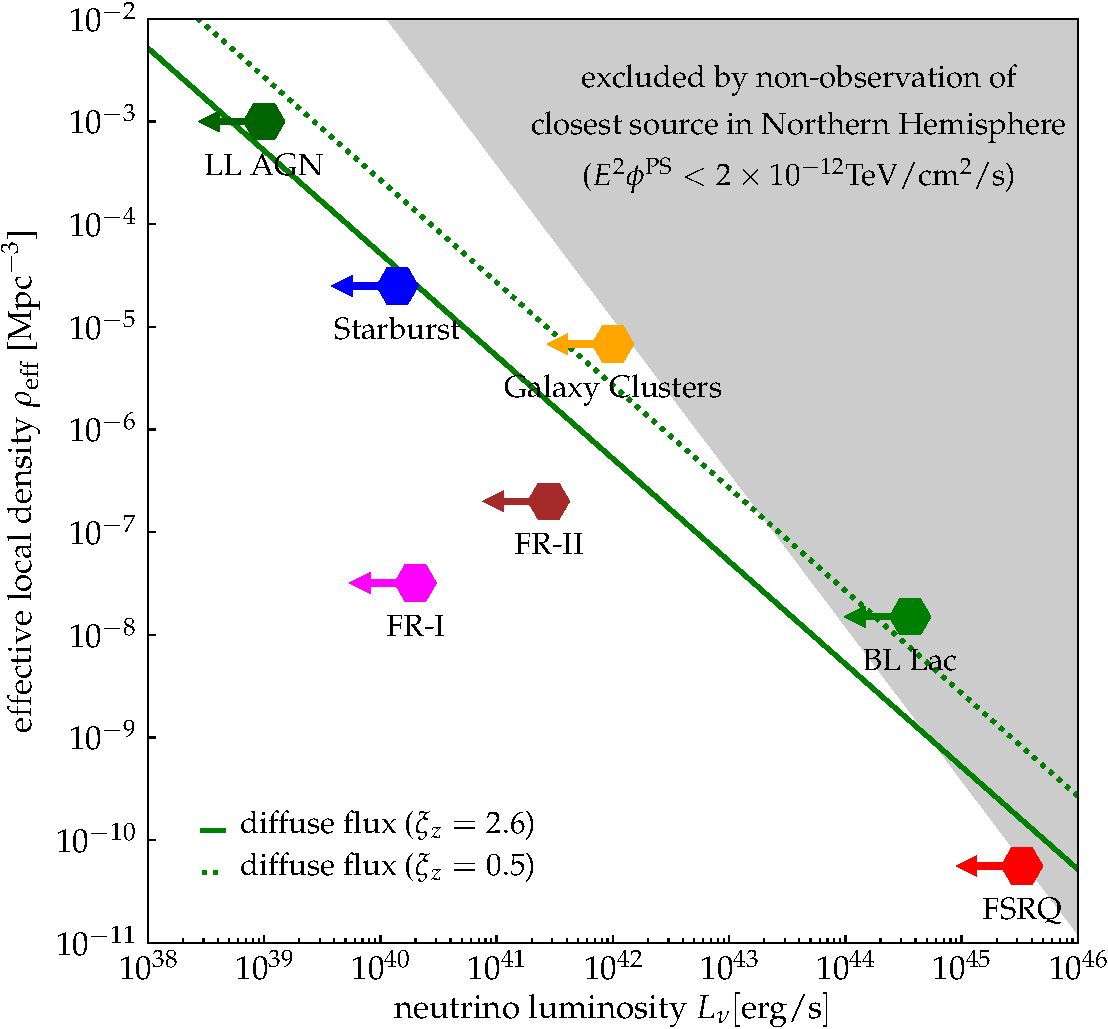
\includegraphics[width=0.5\textwidth]{figures/luminosityDISCOVERY.pdf}
\caption{Alhers Halzen~\cite{Ahlers2018ppnp}}
\end{figure}

Measurements of UHECRs have provided an estimated intensity at a proton energy of \(E_p \gtrsim 10^{17}\) eV as:
%
\[ 
E_p^2 I^{\rm UHE}_p \simeq 10^{-7} \, \text{GeV}~\text{cm}^{-2}~\text{s}^{-1}~\text{sr}^{-1} 
\]

Correspondingly, this implies a cosmic ray luminosity density of:
%
\[ 
E_p^2 \frac{dQ_p}{dV} \simeq 10^{44}~\text{erg}~\text{Mpc}^{-3}~\text{yr}^{-1} 
\]

Using these values, we can infer an upper limit for the production rate of pions:
%
\[
E_{\pi^+} Q_{\pi^+} (E_{\pi^+}) + E_{\pi^0} Q_{\pi^0}(E_{\pi^0}) \simeq \left[E_p Q_p(E_p) \right]_{E_p \simeq E_{\pi} \left\langle {E_p}/{E_{\pi}} \right\rangle}
\]

This relation can be approximated as:
\[
\left(\frac{1 + R_{\pi}}{R_{\pi}} \right) E_{\pi^+} Q_{\pi^+} (E_{\pi^+}) \simeq \left[E_p Q_p(E_p) \right]_{E_p \simeq E_{\pi} \left\langle {E_p}/{E_{\pi}} \right\rangle}
\]
And further refined to:
\[
\left(\frac{1 + R_{\pi}}{R_{\pi}} \right) E^2_{\pi^+} Q_{\pi^+} (E_{\pi^+}) \simeq \frac{1}{\left\langle {E_p}/{E_{\pi}} \right\rangle} \left[E^2_p Q_p(E_p) \right]_{E_p \simeq E_{\pi} \left\langle {E_p}/{E_{\pi}} \right\rangle}
\]

\begin{figure}[!t]
\centering
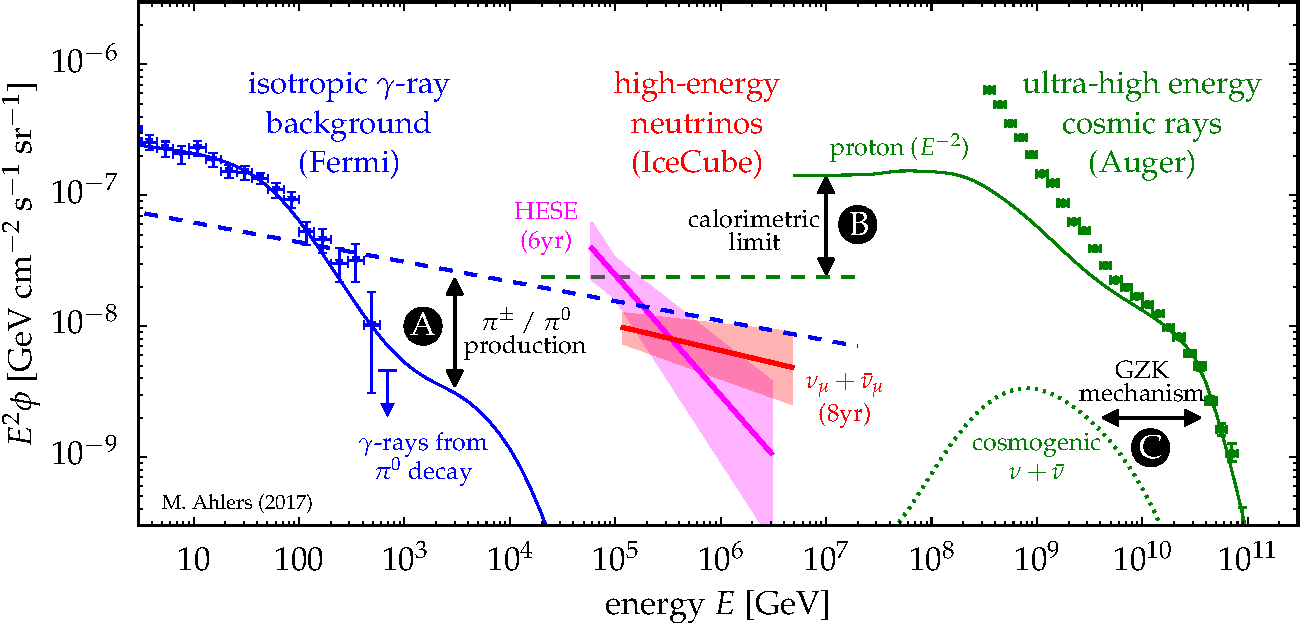
\includegraphics[width=0.90\textwidth]{figures/panorama.pdf}
\caption{Alhers Halzen~\cite{Ahlers2018ppnp}}
\end{figure}

Thus, the refined expression for the pion production rate becomes:
%
\begin{remark}
\[
E^2_{\pi^+} Q_{\pi^+} (E_{\pi^+}) \simeq x_{\pi} \frac{R_{\pi}}{1 + R_{\pi}}  \left[E^2_p Q_p(E_p) \right]_{E_p \simeq E_{\pi} \left\langle {E_p}/{E_{\pi}} \right\rangle}
\]
\end{remark}

Here, \(x_{\pi}\) denotes the average fraction of proton energy that gets converted into the energy of pions.

Integrating the previously derived equations, we obtain a relationship for the cumulative intensity of neutrinos across all flavors:
\[
\frac{1}{3} \sum_\alpha E_\nu^2 I_{\nu_\alpha} \lesssim 3 \times 10^{-8} x_\pi \left( \frac{\xi_z}{2.6} \right)~\text{GeV}~\text{cm}^{-2}~\text{s}^{-1}~\text{sr}^{-1}
\]
Here, \( f_\pi = 1 \) represents the calorimetric limit, also known as the Waxman-Bahcall bound. 

This upper limit is primarily applicable to transparent sources, as the local environment's opacity and the presence of other interaction processes, can also impact the overall neutrino production and escape mechanisms.. {\color{red}Say more...}

%, characterized as follows:
%
%In a transparent source scenario, protons are accelerated within regions containing strong magnetic fields. These protons interact with photons, leading to the generation of both neutral and charged pions. While secondary protons might be confined within the acceleration zone, approximately equal amounts of neutrons, as well as the decay products of both neutral and charged pions, escape. Consequently, the energy exiting the source is partitioned among cosmic rays, gamma rays, and neutrinos—the latter originating from the decay of neutrons, neutral pions, and charged pions.

An underlying assumption for this model is that the source spectrum is steeper than an \(E^{-2}\) energy distribution. This assumption is based on typical observations and theoretical considerations of cosmic ray sources. The steeper spectrum implies that there is a relatively higher abundance of lower-energy particles compared to the higher-energy ones, which influences the overall intensity and energy distribution of emitted particles, including neutrinos.

%It's important to note that these considerations are generalized and might vary with specific astrophysical environments and source characteristics. Additional factors, such as the local environment's opacity and the presence of other interaction processes, can also impact the overall neutrino production and escape mechanisms.